\begin{frame}
\frametitle{Aprendendo \LaTeX{}}
\framesubtitle{}
\centering
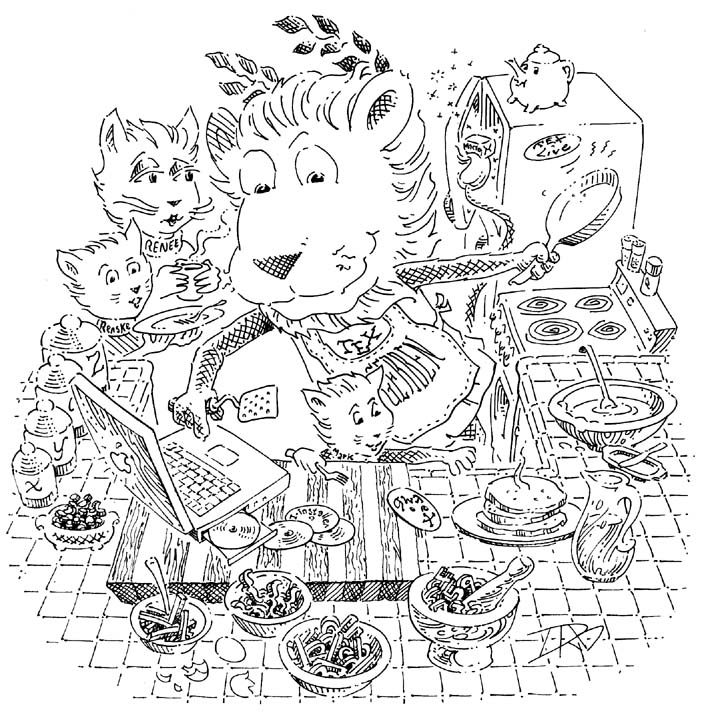
\includegraphics[width=0.7\linewidth]{figures/lion02.png}
\end{frame}



\begin{frame}
\frametitle{Arquivos}
\framesubtitle{Quais arquivos são utilizados?}
\begin{description}
\item[.tex] arquivo fonte do documento \TeX{} ou \LaTeX{} (slide \ref{sec:tex})
\item[.cls] arquivo de classe de documento (slide \ref{clsfile})
\item[.sty] arquivo de estilo, pacotes (slide \ref{clsfile})
\item[.bib] arquivo de bibliografia do BibTeX (slide \ref{bibtex})
\end{description}
\end{frame}

\begin{frame}
\frametitle{Conteúdo e Apresentação}
\framesubtitle{foque em uma coisa de cada vez e diminua o esforço necessário}
  CSS/HTML (web design) e \LaTeX{} (formatação de texto) são exemplos onde empregamos a separação entre conteúdo e forma.
  \begin{figure}[h!]
  \centering
  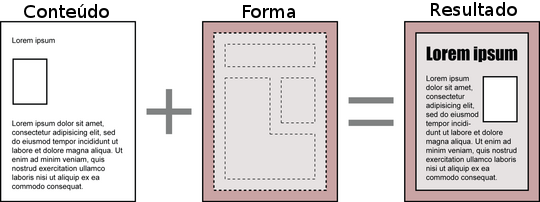
\includegraphics[width=\textwidth]{figures/content_design.png}
  \label{fig:content_design}
  \end{figure}
\end{frame}



\subsection{Arquivo \TeX{}}\label{sec:tex}
\begin{frame}
\frametitle{Arquivo .tex}
\framesubtitle{principal arquivo do seu documento}
O arquivo .tex será o principal arquivo do seu documento. Neste arquivo você incluirá/definirá:
\begin{itemize}
    \item classe do documento
    \item tamanho de fonte, tamanho da página, coluna simples ou dupla, etc
    \item pacotes
    \item texto, figuras, tabelas, equações
    \item outros arquivos .tex
    \item bibliografia
\end{itemize}
\end{frame}


\begin{frame}[fragile]
\frametitle{Espaços em branco}
\framesubtitle{}
  Um ou vários espaços em branco são tratados como um único espaço em branco.
  \scriptsize
  \begin{columns}[c]
  \column{.5\textwidth}
  \begin{verbatim}
Não interessa se introduz apenas
um ou vários     espaços depois
de uma palavra.

Uma linha em branco inicia um novo
parágrafo. 
   \end{verbatim}
  \column{.5\textwidth}
  \begin{fmpage}{\textwidth}
Não interessa se introduz apenas
um ou vários     espaços depois
de uma palavra.

Uma linha em branco inicia um novo
parágrafo.
   \end{fmpage}
   \end{columns}
\end{frame}


\begin{frame}[fragile]
\frametitle{Caracteres reservados}
\framesubtitle{}
Alguns caracteres são reservados:
\begin{verbatim}
#  $  %  ^  &  _  {  }  ~  \ 
\end{verbatim}

Para escrever um desses caracteres é necessário utilizar o caractere de escape.
  \vspace{1cm}
  \scriptsize
  \begin{columns}[c]
  \column{.5\textwidth}
  \begin{verbatim}
  \# \$ \% \^{} \& \_ \{ \} \~{} 
  \textbackslash
   \end{verbatim}
  \column{.5\textwidth}
  \begin{fmpage}{\textwidth}
  \# \$ \% \^{} \& \_ \{ \} \~{}
  \textbackslash
  \end{fmpage}
  \end{columns}
\end{frame}


\begin{frame}[fragile]
\frametitle{Comandos}
\framesubtitle{}
Começam com um backslash e têm um nome que consiste apenas de letras. Os comandos obedecem à seguinte sintaxe:

\begin{verbatim}
\commandname[option1,option2,...]{argument1}{argument2}...
\end{verbatim}

  \scriptsize
  \begin{columns}[c]
  \column{.5\textwidth}
  \begin{verbatim}
Li que o Knuth divide as
pessoas que trabalham com o \TeX{}
em \TeX{}nicos e \TeX pertos.\\
Hoje é \today.
  \end{verbatim}
  \column{.5\textwidth}
  \begin{fmpage}{\textwidth}
Li que o Knuth divide as
pessoas que trabalham com o \TeX{}
em \TeX{}nicos e \TeX pertos.\\
Hoje é \today.
   \end{fmpage}
  \end{columns}
\end{frame}



\begin{frame}[fragile]
\frametitle{Comentários}
\framesubtitle{}
Tudo o que vem após o carácter \% é um comentário. Podemos também fazer comentários em bloco.

  \scriptsize
  \begin{columns}[c]
  \column{.5\textwidth}
  \begin{verbatim}
Este é um % estúpido
% Melhor: instrutivo <----
exemplo: Supercal%
ifragilist%
icexpialidocious
  \end{verbatim}
  \column{.5\textwidth}
  \begin{fmpage}{\textwidth}
Este é um % estúpido
% Melhor: instrutivo <----
exemplo: Supercal%
ifragilist%
icexpialidocious
   \end{fmpage}
  \end{columns}
  \begin{columns}[c]
  \column{.5\textwidth}
  \begin{verbatim}
Este é outro
\begin{comment}
bastante estúpido,
mas instrutivo
\end{comment}
exemplo de como embeber
comentários nos seus documentos.
  \end{verbatim}
  \column{.5\textwidth}
  \begin{fmpage}{\textwidth}
Este é outro
\begin{comment}
bastante estúpido,
mas instrutivo
\end{comment}
exemplo de como embeber
comentários nos seus documentos.
   \end{fmpage}
  \end{columns}
\end{frame}

\begin{frame}[fragile]
\frametitle{Estrutura}
\framesubtitle{}
  A seguinte estrutura é esperada em um arquivo \LaTeX{}.

\begin{verbatim}
\documentclass{...}
\usepackage{...}
...
\begin{document}
...
\end{document}
\end{verbatim}
\end{frame}

\begin{frame}[fragile]
\frametitle{Exemplo}
\framesubtitle{}
  \scriptsize
  \begin{columns}[c]
  \column{.5\textwidth}
\begin{verbatim}
\documentclass{article}
% esta linha é específica para
% o Português e outras línguas
% com caracteres acentuados.
\usepackage[latin1]{inputenc}
\begin{document}
Pequeno é belo.
\end{document}
\end{verbatim}
  \column{.5\textwidth}
  \vspace{-0.3cm}
  \begin{figure}[h!]
  \centering
  \setlength\fboxsep{0pt}
  \setlength\fboxrule{0.5pt}
  \fbox{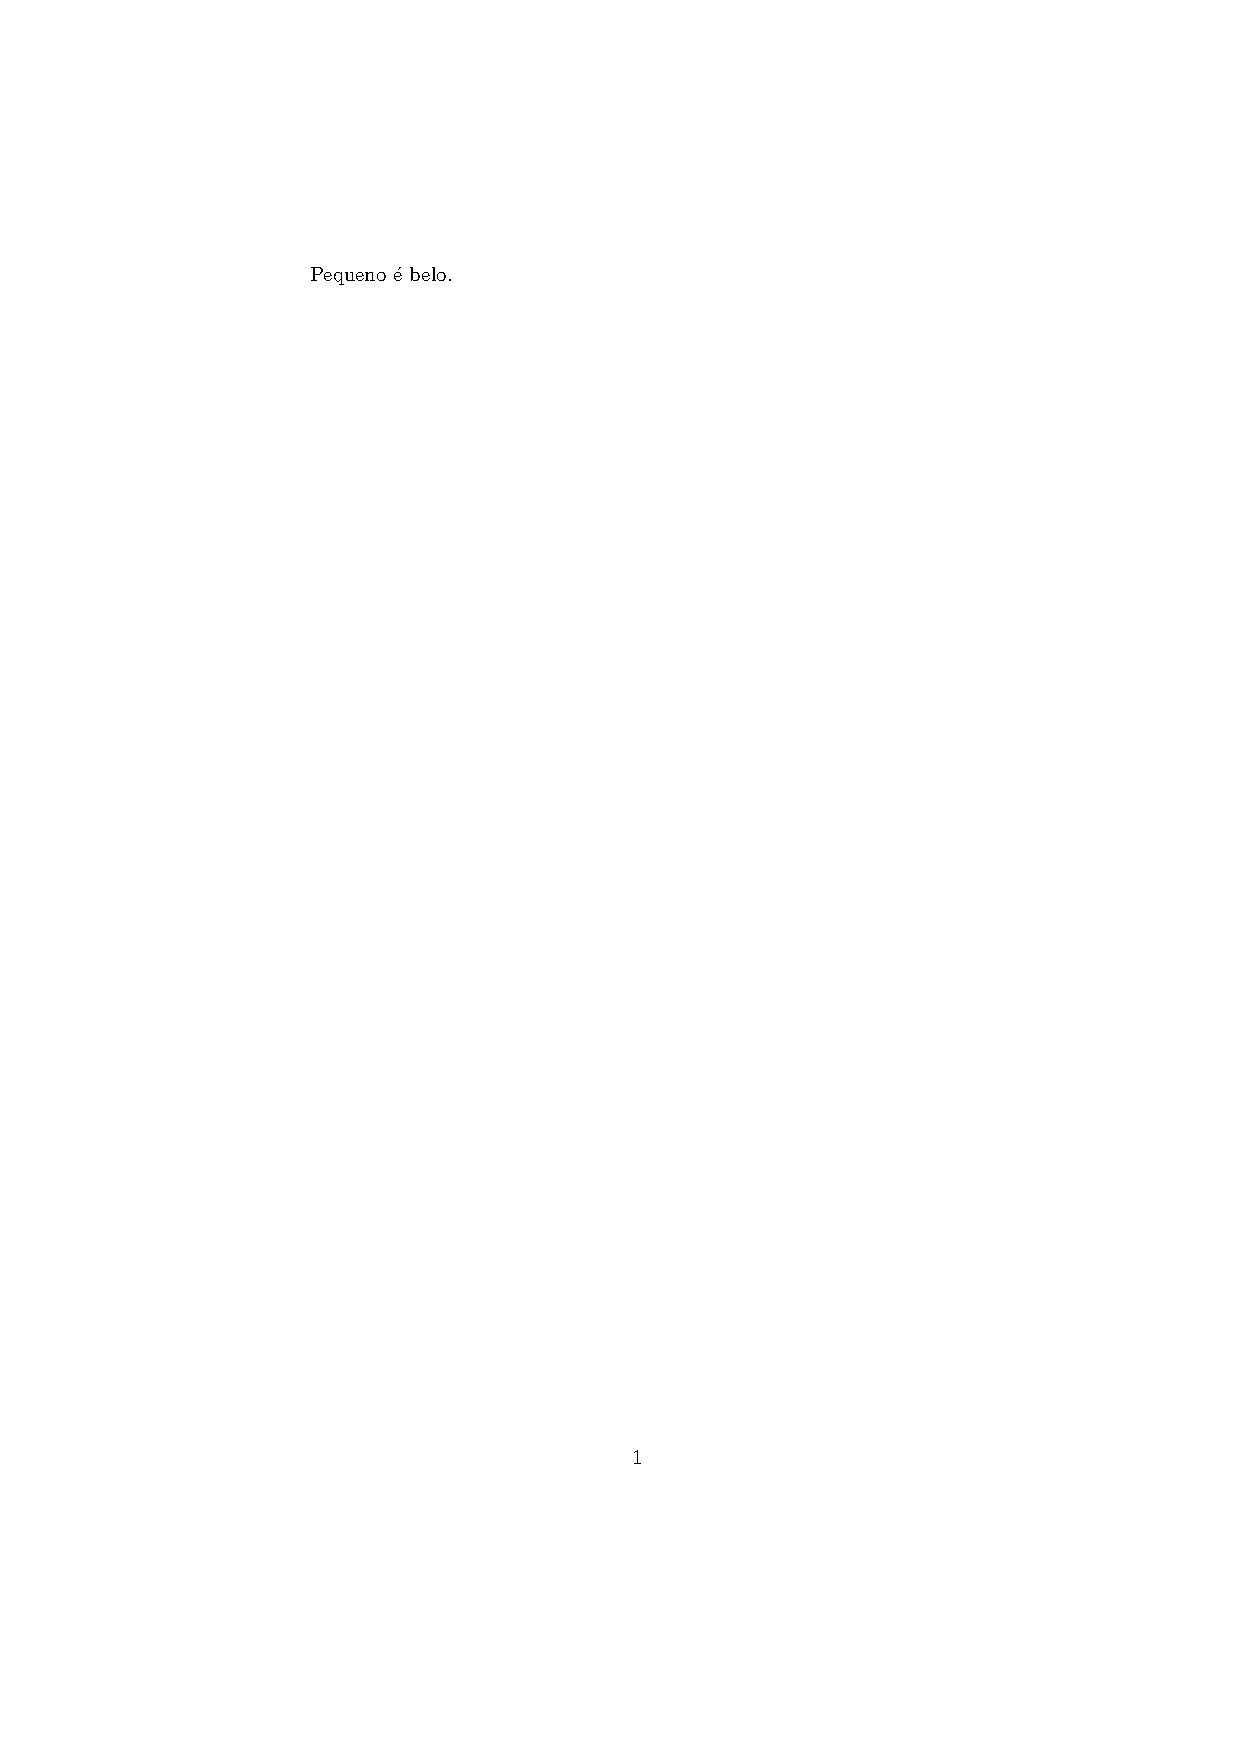
\includegraphics[width=0.8\textwidth]{minimal.pdf}}
  \label{fig:minimal}
  \end{figure}
  \end{columns}
\end{frame}

\begin{frame}[fragile]
\frametitle{Exemplo 2}
\framesubtitle{}
  \scriptsize
  \begin{columns}[c]
  \column{.5\textwidth}
\begin{verbatim}
\documentclass[a4paper,11pt]{article}
% Esta linha é necessária para
% documentos em línguas que incluam
% caracteres acentuados.
\usepackage[latin1]{inputenc}
% Define o autor e título
\author{H.Partl}
\title{Minimalista}
\begin{document}
% Gera o título
\maketitle
% Insere a tabela de conteúdos
\tableofcontents
\section{Algumas Palavras Interessantes}
Bem, e aqui está o inicio do meu adorado artigo.
\section{Adeus, Mundo!}
\ldots{} e aqui ele acaba.
\end{document}
\end{verbatim}
  \column{.5\textwidth}
  \vspace{-0.3cm}
  \begin{figure}[h!]
  \centering
  \setlength\fboxsep{0pt}
  \setlength\fboxrule{0.5pt}
  \fbox{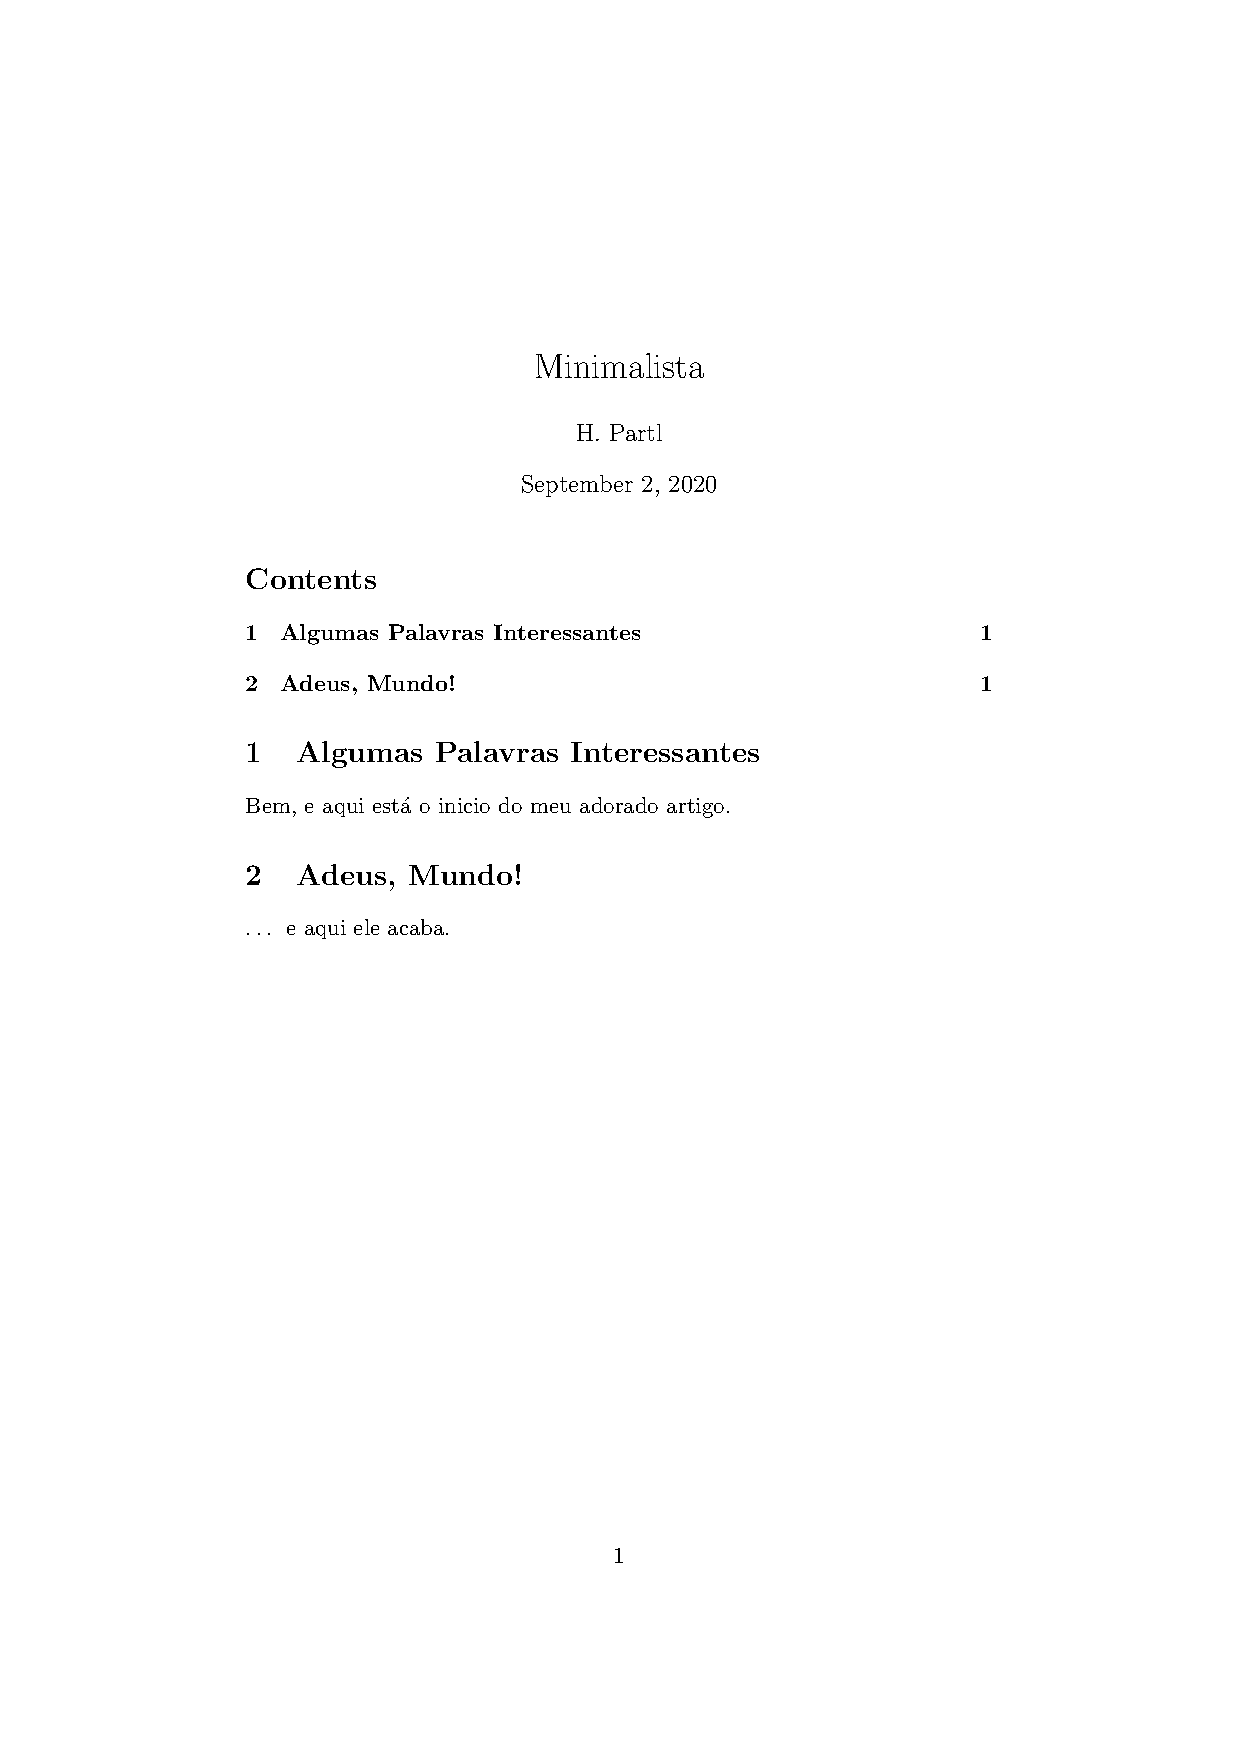
\includegraphics[width=0.8\textwidth]{minimal2.pdf}}
  \label{fig:minimal2}
  \end{figure}
  \end{columns}
\end{frame}

\begin{frame}[fragile]
\frametitle{Documento}
\framesubtitle{classes de documento}
  \begin{verbatim}
  \documentclass[opções]{classe}
  \end{verbatim}
  Exemplo:
  \begin{verbatim}
  \documentclass[11pt,twoside,a4paper]{article}
  \end{verbatim}
  Classes
  \begin{description}
  \item[article] para artigos em jornais científicos, pequenos relatórios, documentação de programas, convites, ...
  \item[report] para relatórios mais longos contendo vários capítulos, pequenos livros, teses de doutorado, ...  
  \item[book] para livros
  \item[slides] para slides. Esta classe usa letras grandes do tipo sans serif. Deve-se
       considerar utilizar o pacote Beamer.
  \end{description}

\end{frame}

\begin{frame}
\frametitle{Documento}
\framesubtitle{atributos dos docuementos}
  Opções:

  \setbeamertemplate{description item}[align left]
  \begin{description}%[labelwidth=\widthof{\bfseries titlepage, notitlepage}]
  \item[10pt, 11pt, 12pt] -- para definir o tamanho da fonte
  \item[a4paper, letterpaper] -- para definir o tamanho do papel
  \item[titlepage, notitlepage] -- especifica se se deve criar uma nova página depois do título do documento ou não
  \item[twocolumn] -- documento em duas colunas
  \item[twoside, oneside] -- impressão frente-verso ou não  
  \item[openright, openany] -- faz os capítulos começarem apenas nas páginas do lado direito ou na próxima disponível
  \item[landscape] -- formato paisagem
  \end{description}

\end{frame}

\begin{frame}[fragile]
\frametitle{Documento}
\framesubtitle{Incluir um documento em outro documento}
  Pomos incluir um arquivo \texttt{.tex} dentro de outro. Para tanto, basta fazer:
  
  \begin{verbatim}
  \input{nome_do_arquivo}
  
  \include{nome_do_arquivo} 
  equivalente a 
  \clearpage \input{nome_do_arquivo} \clearpage
  \end{verbatim}
\end{frame}



\begin{frame}[fragile]
\frametitle{Documento}
\framesubtitle{Comandos de Secção}
  
\begin{verbatim}
\part{}

\chapter{}

\section{}

\subsection{}

\subsubsection{}

\paragraph{}
\end{verbatim}

\end{frame}



\begin{frame}[fragile]
\frametitle{Documento}
\framesubtitle{quebra de linha e nova página}

  \begin{scriptsize}
  \begin{columns}[c]
  \column{.5\textwidth}
  \begin{verbatim}
  você pode \\ quebrar uma linha 
  quando quiser no \newline \LaTeX, 
  entretanto uma simples quebra
  de linha do código não reflete 
  em quebra de linha... 
  
  mas você pode deixar uma linha 
  em branco
  \end{verbatim} 
  \column{.5\textwidth}
  \begin{fmpage}{\textwidth}
  você pode \\ quebrar uma linha 
  quando quiser no \newline \LaTeX, 
  entretanto uma simples quebra
  de linha do código não reflete 
  em quebra de linha... 
  
  mas você pode deixar uma linha 
  em branco
  \end{fmpage}
  \end{columns}
  \end{scriptsize}
  
  Comando utilizado para iniciar uma nova página:
 
  \begin{verbatim}
  \newpage
  \end{verbatim} 

\end{frame}


\begin{frame}[fragile]
\frametitle{Documento}
\framesubtitle{Hifenização de palavras}
  \begin{verbatim}
\hyphenation{lista de palavras}
  \end{verbatim}

  \scriptsize
  \begin{columns}[c]
  \column{.5\textwidth}
  \begin{verbatim}
  \hyphenation{MINICURSOLATEX uni-ver-si-da-de}
  Penso que isto é: su\-per\-cal\-%
  i\-frag\-i\-lis\-tic\-ex\-pi\-%
  al\-i\-do\-cious
  
  Teste de hifenização da palavra 
  universidade, inclusive de  
  certa  palavra MINICURSOLATEX, 
  que não deve ser hifenizada.
  \end{verbatim} 
  \column{.5\textwidth}
  \begin{fmpage}{\textwidth}
  \hyphenation{MINICURSOLATEX uni-ver-si-da-de}
  Penso que isto é: su\-per\-cal\-%
  i\-frag\-i\-lis\-tic\-ex\-pi\-%
  al\-i\-do\-cious
  
  Teste de hifenização da palavra 
  universidade, inclusive de  
  certa  palavra MINICURSOLATEX, 
  que não deve ser hifenizada.
  \end{fmpage}
  \end{columns}
\end{frame}


\begin{frame}[fragile]
\frametitle{Documento}
\framesubtitle{Estilo de fonte em um texto}
  \begin{columns}[c]
  \column{.5\textwidth}
  \begin{verbatim}
  \textbf{Bold} \\
  \textit{Italic} \\
  \texttt{Monotype} \\
  \textsf{Sans Serif} \\
  \textsc{SmallCaps} \\
  \textsl{Slanted} \\
  \emph{Enfase}
  \end{verbatim} 
  \column{.5\textwidth}
  \begin{fmpage}{\textwidth}
  \textbf{Bold} \\
  \textit{Italic} \\
  \texttt{Monotype} \\
  \textsf{Sans Serif} \\
  \textsc{SmallCaps} \\
  \textsl{Slanted} \\
  \emph{Enfase}
  \end{fmpage}
  \end{columns}
\end{frame}


\begin{frame}[fragile]
\frametitle{Documento}
\framesubtitle{Tamanho da fonte em um texto}
  \begin{columns}[c]
  \column{.5\textwidth}
  \scriptsize
  \begin{verbatim}
  {\tiny texto texto ...} \\
  {\scriptsize texto texto ...} \\
  {\footnotesize texto texto ...} \\
  {\small texto texto ...} \\
  {\normalsize texto texto ...} \\
  {\large texto texto ...} \\
  {\Large texto texto ...} \\
  {\LARGE texto texto ...} \\
  {\huge texto texto ...} \\
  {\Huge texto texto ...}
  \end{verbatim} 
  \column{.5\textwidth}
  \begin{fmpage}{\textwidth}
  {\tiny texto texto ...} \\
  {\scriptsize texto texto ...} \\
  {\footnotesize texto texto ...} \\
  {\small texto texto ...} \\
  {\normalsize texto texto ...} \\
  {\large texto texto ...} \\
  {\Large texto texto ...} \\
  {\LARGE texto texto ...} \\
  {\huge texto texto ...} \\
  {\Huge texto texto ...}
  \end{fmpage}
  \end{columns}
\end{frame}

\begin{frame}[fragile]
\frametitle{Documento}
\framesubtitle{Alinhamento de texto}
  \scriptsize
  \begin{columns}[c]
  \column{.5\textwidth}
  \begin{verbatim}
  \begin{center}
  texto texto
  \end{center}
  \begin{flushleft}
  texto texto
  \end{flushleft}
  \begin{flushright}
  texto texto
  \end{flushright}
  \end{verbatim} 
  \column{.5\textwidth}
  \begin{fmpage}{\textwidth}
  \begin{center}
  texto texto
  \end{center}
  \begin{flushleft}
  texto texto
  \end{flushleft}
  \begin{flushright}
  texto texto
  \end{flushright}
  \end{fmpage}
  \end{columns}
\end{frame}

\begin{frame}[fragile]
\frametitle{Documento}
\framesubtitle{Layout de uma página}
  \scriptsize
  \begin{columns}[c]
  \column{.5\textwidth}
  \begin{itemize}
  \item \verb|\hoffset|
  \item \verb|\voffset|
  \item \verb|\oddsidemargin|
  \item \verb|\topmargin|
  \item \verb|\headheight|
  \item \verb|\headsep|
  \item \verb|\textheight| 
  \item \verb|\textwidth|
  \item \verb|\marginparsep|
  \item \verb|\marginparwidth|
  \item \verb|\footskip|
  \end{itemize}
  \column{.5\textwidth}
  \vspace{-1.5cm}
\begin{figure}[h!]
  \centering
  \label{fig:Latex_layout}
    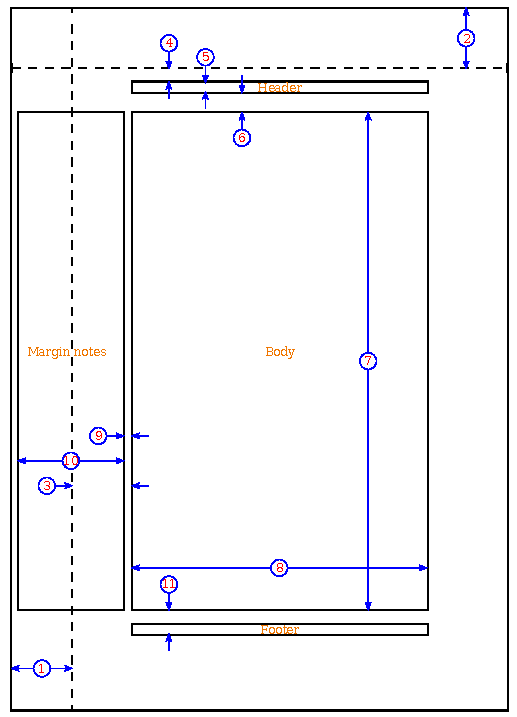
\includegraphics[width=0.85\textwidth]{figures/Latex_layout.pdf}
  %\caption{Tux.}
\end{figure}
  \end{columns}
\end{frame}


\begin{frame}[fragile]
\frametitle{Documento}
\framesubtitle{Layout}
  \scriptsize
  \begin{verbatim}
%\documentclass[a4paper]{article}
%\usepackage[top=tlength, bottom=blength, left=llength,
%        right=rlength]{geometry}
%\usepackage[a4paper,landscape]{geometry}
  \end{verbatim} 
\end{frame}


\begin{frame}[fragile]
\frametitle{Documento}
\framesubtitle{Cabeçalho e Rodapé}
  \scriptsize
  \begin{verbatim}
\usepackage{fancyhdr}

\fancyhead[CE]{Author's Name}
\fancyhead[CO]{\today}
\fancyfoot[LE,RO]{\thepage}
  \end{verbatim} 
  
  \url{https://ctan.org/pkg/fancyhdr} \\
  \url{https://www.overleaf.com/learn/latex/Headers_and_footers}
\end{frame}


\begin{frame}[fragile]
\frametitle{Documento}
\framesubtitle{misturar coluna simples com multiplas colunas}
\scriptsize
\begin{verbatim}
\begin{multicols}{2}
  lots of text
\end{multicols}
\end{verbatim} 

\url{https://www.ctan.org/pkg/multicol} \\
\url{https://www.overleaf.com/learn/latex/Multiple_columns}
\end{frame}


\begin{frame}[fragile]
\frametitle{Documento}
\framesubtitle{Nota s de rodapé}
  \scriptsize
  \begin{columns}[c]
  \column{.5\textwidth}
  \begin{verbatim}
Exemplo de nota de rodapé
\footnote{Isto é uma nota de rodapé.}.
  \end{verbatim} 
  \column{.5\textwidth}
  \begin{fmpage}{\textwidth}
  Exemplo de nota de rodapé\footnote{Isto é uma nota de rodapé.}.
  \vspace{5cm}
  \end{fmpage}
  \end{columns}
\end{frame}

\begin{frame}[fragile]
\frametitle{Documento}
\framesubtitle{Sumário}
  \scriptsize
  \begin{columns}[c]
  \column{.5\textwidth}
  \begin{verbatim}
\tableofcontents
  \end{verbatim} 
  \column{.5\textwidth}
  \begin{fmpage}{\textwidth}
  \scriptsize
  \tableofcontents
  \end{fmpage}
  \end{columns}
\end{frame}


\begin{frame}[fragile]
\frametitle{Documento}
\framesubtitle{Sumário - local corrente}
  \scriptsize
  \begin{columns}[c]
  \column{.5\textwidth}
  \begin{verbatim}
\tableofcontents[current,currentsection]
  \end{verbatim} 
  \column{.5\textwidth}
  \begin{fmpage}{\textwidth}
  \scriptsize
  \tableofcontents[current,currentsection]
  \end{fmpage}
  \end{columns}
\end{frame}


\subsection{Listas}\label{sec:listas}
\begin{frame}[fragile]
\frametitle{Documento}
\framesubtitle{Lista de itens}
  \scriptsize
  \begin{columns}[c]
  \column{.5\textwidth}
  \begin{verbatim}
  \begin{itemize}
  \item item 1
  \item item 2
  \item item 3
  \end{itemize}
  \end{verbatim}
  \column{.5\textwidth}
  \begin{fmpage}{\textwidth}
  \begin{itemize}
  \item item 1
  \item item 2
  \item item 3
  \end{itemize}
  \end{fmpage}
  \end{columns}
\end{frame}



\begin{frame}[fragile]
\frametitle{Documento}
\framesubtitle{Lista numerada}
  \scriptsize
  \begin{columns}[c]
  \column{.5\textwidth}
  \begin{verbatim}
  \begin{enumerate}
  \item item 1
  \item item 2
  \item item 3
  \end{enumerate}
  \end{verbatim}
  \column{.5\textwidth}
  \begin{fmpage}{\textwidth}
  \begin{enumerate}
  \item item 1
  \item item 2
  \item item 3
  \end{enumerate}
  \end{fmpage}
  \end{columns}
\end{frame}



\begin{frame}[fragile]
\frametitle{Documento}
\framesubtitle{Listas encadeadas}
  \scriptsize
  \begin{columns}[c]
  \column{.5\textwidth}
  \begin{verbatim}
  \begin{enumerate}
  \item item 1
    \begin{itemize}
    \item item 1.1
    \item item 1.2
    \item item 1.3
    \end{itemize}
  \item item 2
  \item item 3
  \end{enumerate}
  \end{verbatim}
  \column{.5\textwidth}
  \begin{fmpage}{\textwidth}
  \begin{enumerate}
  \item item 1
    \begin{itemize}
    \item item 1.1
    \item item 1.2
    \item item 1.3
    \end{itemize}
  \item item 2
  \item item 3
  \end{enumerate}
  \end{fmpage}
  \end{columns}
\end{frame}


\begin{frame}[fragile]
\frametitle{Documento}
\framesubtitle{Lista encadeada}
  \scriptsize
  \begin{columns}[c]
  \column{.5\textwidth}
  \begin{verbatim}
  \begin{enumerate}
  \item item 1
    \begin{enumerate}[a)]
    \item item 1.1
    \item item 1.2
    \item item 1.3
    \end{enumerate}
  \item item 2
  \item item 3
  \end{enumerate}
  \end{verbatim}
  \column{.5\textwidth}
  \begin{fmpage}{\textwidth}
  \begin{enumerate}
  \item item 1
    \begin{enumerate}[a)]
    \item item 1.1
    \item item 1.2
    \item item 1.3
    \end{enumerate}
  \item item 2
  \item item 3
  \end{enumerate}
  \end{fmpage}
  \end{columns}
\end{frame}


\begin{frame}[fragile]
\frametitle{Documento}
\framesubtitle{}
  \scriptsize
  \begin{columns}[c]
  \column{.5\textwidth}
  \begin{verbatim}
  \begin{description}
  \item[primeiro item] item 1
  \item[segundo item] item 2
  \item[terceiro item] item 3
  \end{description}
  \end{verbatim}
  \column{.5\textwidth}
  \begin{fmpage}{\textwidth}
  \begin{description}
  \item[primeiro item] txt1 txt1 txt1
  \item[segundo item] txt2 txt2 txt2
  \item[terceiro item] txt3 txt3 txt3
  \end{description}
  \end{fmpage}
  \end{columns}
\end{frame}


\begin{frame}[fragile]
\frametitle{Documento}
\framesubtitle{mais sobre listas}
\url{https://en.wikibooks.org/wiki/LaTeX/List_Structures}
\url{https://www.overleaf.com/learn/latex/Lists}
\end{frame}

\subsection{Figuras}\label{sec:figuras}
\begin{frame}[fragile]
\frametitle{Documento}
\framesubtitle{Como inserir uma figura no documento}
  \scriptsize
  \begin{columns}[c]
  \column{.5\textwidth}
  \begin{verbatim}
\begin{figure}[h!]
  \centering
  \label{fig:tux}
  
\includegraphics[width=0.5\textwidth]
                     {334px-tuxsvg.png}
  \caption{Tux.}
\end{figure}
  \end{verbatim}
  \column{.5\textwidth}
  \begin{fmpage}{\textwidth}
\begin{figure}[h!]
  \centering
  \label{fig:tux}
    
\includegraphics[width=0.5\textwidth]{figures/334px-tuxsvg.png}
  \caption{Tux.}
\end{figure}
  \end{fmpage}
  \end{columns}
\end{frame}


\begin{frame}[fragile]
\frametitle{Documento}
\framesubtitle{Referenciando uma figura no texto}
  \scriptsize
  \begin{columns}[c]
  \column{.5\textwidth}
  \begin{verbatim}
  Veja a Figura \ref{fig:tux} 
  na página \pageref{fig:tux}.
  \end{verbatim}
  \column{.5\textwidth}
  \begin{fmpage}{\textwidth}
  Veja a Figura \ref{fig:tux} na página \pageref{fig:tux}.
  \end{fmpage}
  \end{columns}
\end{frame}


\begin{frame}[fragile]
\frametitle{Documento}
\framesubtitle{Subfiguras}
  \scriptsize
  \begin{columns}[c]
  \column{.5\textwidth}
  \begin{verbatim}
\begin{figure}[ht]
\centering
\subfigure[Tux 1]{
   
\includegraphics[width=0.3\textwidth] 
              {figures/334px-tuxsvg.png}
   \label{fig:tux1}
 }
 \subfigure[Tux 2]{
   
\includegraphics[width=0.3\textwidth] 
                      {figures/tux2.png}
   \label{fig:tux2}
 }
\caption{Linux Tux.}
\end{figure}
  \end{verbatim}
  \column{.5\textwidth}
  \begin{fmpage}{\textwidth}
\begin{figure}[ht]
\centering
\subfigure[Tux 1]{
   
\includegraphics[width=0.3\textwidth] {figures/334px-tuxsvg.png}
   \label{fig:tux1}
 }
 \subfigure[Tux 2]{
   
\includegraphics[width=0.3\textwidth] {figures/tux2.png}
   \label{fig:tux2}
 }
\caption{Linux Tux.}
\end{figure}
  \end{fmpage}
  \end{columns}
\end{frame}


\begin{frame}[fragile]
\frametitle{Documento}
\framesubtitle{referenciando as figuras}
  \scriptsize
  \begin{columns}[c]
  \column{.5\textwidth}
  \begin{verbatim}
  Veja as subfiguras \ref{fig:tux1} 
  e \ref{fig:tux2} na página 
  \pageref{fig:tux1}.
  \end{verbatim}
  \column{.5\textwidth}
  \begin{fmpage}{\textwidth}
  Veja as subfiguras \ref{fig:tux1} e \ref{fig:tux2} na página \pageref{fig:tux1}.
  \end{fmpage}
  \end{columns}
\end{frame}


\subsection{Tabelas}\label{sec:tabelas}
\begin{frame}[fragile]
\frametitle{Documento}
\framesubtitle{Tabela simples}
  \scriptsize
  \begin{columns}[c]
  \column{.5\textwidth}
  \begin{verbatim}
  \begin{tabular}{ l c r }
  1 & 2 & 3 \\
  4 & 5 & 6 \\
  7 & 8 & 9 \\
  \end{tabular}
  \end{verbatim}
  \column{.5\textwidth}
  \begin{fmpage}{\textwidth}
  \begin{tabular}{ l c r }
  1 & 2 & 3 \\
  4 & 5 & 6 \\
  7 & 8 & 9 \\
  \end{tabular}
  \end{fmpage}
  \end{columns}
\end{frame}


\begin{frame}[fragile]
\frametitle{Documento}
\framesubtitle{Tabela}
  \scriptsize
  \begin{columns}[c]
  \column{.5\textwidth}
  \begin{verbatim}
\begin{tabular}{ l | c || r | }
  1 & 2 & 3 \\
  4 & 5 & 6 \\
  7 & 8 & 9 \\
\end{tabular}
  \end{verbatim}
  \column{.5\textwidth}
  \begin{fmpage}{\textwidth}
\begin{tabular}{ l | c || r | }
  1 & 2 & 3 \\
  4 & 5 & 6 \\
  7 & 8 & 9 \\
\end{tabular}
  \end{fmpage}
  \end{columns}
\end{frame}


\begin{frame}[fragile]
\frametitle{Documento}
\framesubtitle{Tabela}
  \scriptsize
  \begin{columns}[c]
  \column{.5\textwidth}
  \begin{verbatim}
\begin{center}
  \begin{tabular}{ l | c || r | }
    \hline
    1 & 2 & 3 \\ \hline
    4 & 5 & 6 \\ \hline
    7 & 8 & 9 \\
    \hline
  \end{tabular}
\end{center}
  \end{verbatim}
  \column{.5\textwidth}
  \begin{fmpage}{\textwidth}
\begin{center}
  \begin{tabular}{ l | c || r | }
    \hline
    1 & 2 & 3 \\ \hline
    4 & 5 & 6 \\ \hline
    7 & 8 & 9 \\
    \hline
  \end{tabular}
\end{center}
  \end{fmpage}
  \end{columns}
\end{frame}


\begin{frame}[fragile]
\frametitle{Documento}
\framesubtitle{Uma tabela um pouco mais complexa}
  \scriptsize
  \begin{columns}[c]
  \column{.5\textwidth}
  \begin{verbatim}
\begin{tabular}{|r|l|}
  \hline
  7C0 & hexadecimal \\
  3700 & octal \\ \cline{2-2}
  11111000000 & binary \\
  \hline \hline
  1984 & decimal \\
  \hline
\end{tabular}
  \end{verbatim}
  \column{.5\textwidth}
  \begin{fmpage}{\textwidth}
\begin{tabular}{|r|l|}
  \hline
  7C0 & hexadecimal \\
  3700 & octal \\ \cline{2-2}
  11111000000 & binary \\
  \hline \hline
  1984 & decimal \\
  \hline
\end{tabular}
  \end{fmpage}
  \end{columns}
\end{frame}


\begin{frame}[fragile]
\frametitle{Documento}
\framesubtitle{uma tabela maior}
\scriptsize
  podemos definir várias colunas de uma vez utilizando a sintaxe:
  \vspace{-0.2cm}
  \begin{verbatim}
  *{num}{str}
  \end{verbatim}
  %\begin{columns}[c]
  %\column{.5\textwidth}
  \vspace{-0.5cm}
  \begin{verbatim}
\begin{tabular}{l*{6}{c}r}
Team              & P & W & D & L & F  & A & Pts \\
\hline
Manchester United & 6 & 4 & 0 & 2 & 10 & 5 & 12  \\
Celtic            & 6 & 3 & 0 & 3 &  8 & 9 &  9  \\
Benfica           & 6 & 2 & 1 & 3 &  7 & 8 &  7  \\
FC Copenhagen     & 6 & 2 & 1 & 2 &  5 & 8 &  7  \\
\end{tabular}
  \end{verbatim}
  %\column{.5\textwidth}
  \vspace{-0.2cm}
  \begin{fmpage}{\textwidth}
\begin{tabular}{l*{6}{c}r}
Team              & P & W & D & L & F  & A & Pts \\
\hline
Manchester United & 6 & 4 & 0 & 2 & 10 & 5 & 12  \\
Celtic            & 6 & 3 & 0 & 3 &  8 & 9 &  9  \\
Benfica           & 6 & 2 & 1 & 3 &  7 & 8 &  7  \\
FC Copenhagen     & 6 & 2 & 1 & 2 &  5 & 8 &  7  \\
\end{tabular}
\end{fmpage}
\end{frame}


\begin{frame}[fragile]
\frametitle{Documento}
\framesubtitle{}
  \scriptsize
  quebra (wrapping) de texto e largura fixa
  \vspace{-0.2cm}
  \scriptsize
  \begin{verbatim}
    \begin{tabular}{ | l | l | l | p{5cm} |}
    \hline
    Day & Min Temp & Max Temp & Summary \\ \hline
    Monday & 11C & 22C & A clear day with lots of sunshine.  
    However, the strong breeze will bring down the temperatures. \\ \hline
    Tuesday & 9C & 19C & Cloudy with rain, across many northern regions. Clear spells
    across most of Scotland and Northern Ireland,
    but rain reaching the far northwest. \\
    \hline
    \end{tabular}
  \end{verbatim}
  \vspace{-0.2cm}
  \begin{fmpage}{\textwidth}
    \begin{tabular}{ | l | l | l | p{5cm} |}
    \hline
    Day & Min Temp & Max Temp & Summary \\ \hline
    Monday & 11C & 22C & A clear day with lots of sunshine.
    However, the strong breeze will bring down the temperatures. \\ \hline
    Tuesday & 9C & 19C & Cloudy with rain, across many northern regions. Clear spells
    across most of Scotland and Northern Ireland,
    but rain reaching the far northwest. \\
    \hline
    \end{tabular}
  \end{fmpage}
\end{frame}


\begin{frame}[fragile]
\frametitle{Documento}
\framesubtitle{múltiplas colunas}
  \scriptsize 
  linha/célula ocupando mais de uma coluna
  \begin{columns}[c]
  \column{.5\textwidth}
  \begin{verbatim}
\begin{tabular}{|l|l|}
  \hline
  \multicolumn{2}{|c|}{Team sheet} \\
  \hline
  GK & Paul Robinson \\
  LB & Lucus Radebe \\
  DC & Michael Duberry \\
  DC & Dominic Matteo \\
  RB & Didier Domi \\
  MC & David Batty \\
  MC & Eirik Bakke \\
  MC & Jody Morris \\
  FW & Jamie McMaster \\
  ST & Alan Smith \\
  ST & Mark Viduka \\
  \hline
\end{tabular}
  \end{verbatim}
  \column{.5\textwidth}
  \begin{fmpage}{\textwidth}
\begin{tabular}{|l|l|}
  \hline
  \multicolumn{2}{|c|}{Team sheet} \\
  \hline
  GK & Paul Robinson \\
  LB & Lucus Radebe \\
  DC & Michael Duberry \\
  DC & Dominic Matteo \\
  RB & Didier Domi \\
  MC & David Batty \\
  MC & Eirik Bakke \\
  MC & Jody Morris \\
  FW & Jamie McMaster \\
  ST & Alan Smith \\
  ST & Mark Viduka \\
  \hline
\end{tabular}
  \end{fmpage}
  \end{columns}
\end{frame}


\begin{frame}[fragile]
\frametitle{Documento}
\framesubtitle{múltiplas linhas}
  \scriptsize 
  colunas/células ocupando multiplas linhas \verb|\usepackage{multirow}|
  \begin{columns}[c]
  \column{.5\textwidth}
  \vspace{-0.2cm}
  \scriptsize
  \begin{verbatim}
\begin{tabular}{|l|l|l|}
\hline
\multicolumn{3}{|c|}{Team sheet} \\
\hline
Goalkeeper & GK & Paul Rob. \\ \hline
\multirow{4}{*}{Defenders} & 
         LB & Lucus Radebe \\
 & DC & Michael Duberry \\
 & DC & Dominic Matteo \\
 & RB & Didier Domi \\ \hline
\multirow{3}{*}{Midfielders} & 
           MC & David Batty \\
 & MC & Eirik Bakke \\
 & MC & Jody Morris \\ \hline
Forward & FW & Jamie McMaster \\ \hline
\multirow{2}{*}{Strikers} & 
         ST & Alan Smith \\
 & ST & Mark Viduka \\  \hline
\end{tabular}
  \end{verbatim}
  \column{.5\textwidth}
  \begin{fmpage}{\textwidth}
\begin{tabular}{|l|l|l|}
\hline
\multicolumn{3}{|c|}{Team sheet} \\
\hline
Goalkeeper & GK & Paul Robinson \\ \hline
\multirow{4}{*}{Defenders} & LB & Lucus Radebe \\
 & DC & Michael Duberry \\
 & DC & Dominic Matteo \\
 & RB & Didier Domi \\ \hline
\multirow{3}{*}{Midfielders} & MC & David Batty \\
 & MC & Eirik Bakke \\
 & MC & Jody Morris \\ \hline
Forward & FW & Jamie McMaster \\ \hline
\multirow{2}{*}{Strikers} & ST & Alan Smith \\
 & ST & Mark Viduka \\
\hline
\end{tabular}
  \end{fmpage}
  \end{columns}
\end{frame}


\begin{frame}[fragile]
\frametitle{Documento}
\framesubtitle{cores em uma tabela}
  \scriptsize 
  aplicando cores alternadas às linhas de uma tabela \verb|\usepackage[table]{xcolor}|
  \begin{columns}[c]
  \column{.5\textwidth}
  \vspace{-0.2cm}
  \scriptsize
  \begin{verbatim}
\rowcolors{1}{green}{yellow}

\begin{tabular}{lll}
odd     & odd   & odd \\
even    & even  & even\\
odd     & odd   & odd \\
even    & even  & even\\
\end{tabular}
  \end{verbatim}
  \column{.5\textwidth}
  \begin{fmpage}{\textwidth}
\rowcolors{1}{green}{yellow}

\begin{tabular}{lll}
odd     & odd   & odd \\
even    & even  & even\\
odd     & odd   & odd \\
even    & even  & even\\
\end{tabular}
  \end{fmpage}
  \end{columns}
\end{frame}


\begin{frame}[fragile]
\frametitle{Documento}
\framesubtitle{referências}
\url{https://pt.overleaf.com/learn/latex/Tables}
\url{https://en.wikibooks.org/wiki/LaTeX/Tables}
\end{frame}




\subsection{Fórmulas Matemáticas}\label{sec:formulasmat}
\begin{frame}[fragile]
\frametitle{Documento}
\framesubtitle{Fórmulas}
  \begin{verbatim}
\usepackage{amsmath}
ou
\usepackage{mathtools}
  \end{verbatim}

  Como inserir fórmulas?
  \begin{itemize}
  \item \begin{verbatim}
\( ... \)  ou  $ ... $
        \end{verbatim}
  \item \begin{verbatim}
\begin{equation} ... \end{equation}
        \end{verbatim}
  \end{itemize}
\end{frame}


\begin{frame}[fragile]
\frametitle{Documento}
\framesubtitle{Fórmulas}
  \scriptsize
  \begin{columns}[c]
  \column{.5\textwidth}
  \begin{verbatim}
\begin{equation}
\forall x \in X, 
\quad \exists y \leq \epsilon
\end{equation}
  \end{verbatim}
  \column{.5\textwidth}
  \begin{fmpage}{\textwidth}
\begin{equation}
\forall x \in X, 
\quad \exists y \leq \epsilon
\end{equation}
  \end{fmpage}
  \end{columns}

  \begin{columns}[c]
  \column{.5\textwidth}
  \begin{verbatim}
\begin{equation}
\alpha, \beta, \gamma, \delta,
\epsilon, \zeta, \eta, \theta,
\Gamma, \Delta, \Theta, \Lambda
\pi, \Pi, \phi, \Phi
\end{equation}
  \end{verbatim}
  \column{.5\textwidth}
  \begin{fmpage}{\textwidth}
\begin{equation}
\alpha, \beta, \gamma, \delta,
\epsilon, \zeta, \eta, \theta,
\Gamma, \Delta, \Theta, \Lambda
\pi, \Pi, \phi, \Phi
\end{equation}
  \end{fmpage}
  \end{columns}


  \begin{columns}[c]
  \column{.5\textwidth}
  \begin{verbatim}
\begin{equation}
\cos (2\theta) = 
\cos^2 \theta - \sin^2 \theta
\end{equation}
  \end{verbatim}
  \column{.5\textwidth}
  \begin{fmpage}{\textwidth}
\begin{equation}
\cos (2\theta) = 
\cos^2 \theta - \sin^2 \theta
\end{equation}
  \end{fmpage}
  \end{columns}
\end{frame}


\begin{frame}[fragile]
\frametitle{Documento}
\framesubtitle{Fórmulas}
  \scriptsize
  \begin{columns}[c]
  \column{.5\textwidth}
  \begin{verbatim}
\begin{equation}
\lim_{x \to \infty} \exp(-x) = 0
\end{equation}
  \end{verbatim}
  \column{.5\textwidth}
  \begin{fmpage}{\textwidth}
\begin{equation}
\lim_{x \to \infty} \exp(-x) = 0
\end{equation}
  \end{fmpage}
  \end{columns}


  \begin{columns}[c]
  \column{.5\textwidth}
  \begin{verbatim}
\begin{equation}
a \bmod b
\end{equation}
  \end{verbatim}
  \column{.5\textwidth}
  \begin{fmpage}{\textwidth}
\begin{equation}
a \bmod b
\end{equation}
  \end{fmpage}
  \end{columns}


  \begin{columns}[c]
  \column{.5\textwidth}
  \begin{verbatim}
\begin{equation}
x \equiv a \pmod b
\end{equation}
  \end{verbatim}
  \column{.5\textwidth}
  \begin{fmpage}{\textwidth}
\begin{equation}
x \equiv a \pmod b
\end{equation}
  \end{fmpage}
  \end{columns}
\end{frame}


\begin{frame}[fragile]
\frametitle{Documento}
\framesubtitle{Fórmulas}
  \scriptsize
  \begin{columns}[c]
  \column{.5\textwidth}
  \begin{verbatim}
\begin{equation}
k_{n+1} = n^2 + k_n^2 - k_{n-1}
\end{equation}
  \end{verbatim}
  \column{.5\textwidth}
  \begin{fmpage}{\textwidth}
\begin{equation}
k_{n+1} = n^2 + k_n^2 - k_{n-1}
\end{equation}
  \end{fmpage}
  \end{columns}


  \begin{columns}[c]
  \column{.5\textwidth}
  \begin{verbatim}
\begin{equation}
f(n) = n^5 + 4n^2 + 2 |_{n=17}
\end{equation}
  \end{verbatim}
  \column{.5\textwidth}
  \begin{fmpage}{\textwidth}
\begin{equation}
f(n) = n^5 + 4n^2 + 2 |_{n=17}
\end{equation}
  \end{fmpage}
  \end{columns}


  \begin{columns}[c]
  \column{.5\textwidth}
  \begin{verbatim}
\begin{equation}
(\cdot), [\cdot], \{\cdot\}, |\cdot|, 
\lVert\cdot\rVert, \langle\cdot\rangle, 
\lfloor\cdot\rfloor, \lceil\cdot\rceil
\end{equation}
  \end{verbatim} 
  \column{.5\textwidth}
  \begin{fmpage}{\textwidth}
\begin{equation}
(\cdot), [\cdot], \{\cdot\}, |\cdot|, \lVert\cdot\rVert, \langle\cdot\rangle, \lfloor\cdot\rfloor, \lceil\cdot\rceil
\end{equation}
  \end{fmpage}
  \end{columns}
\end{frame}


\begin{frame}[fragile]
\frametitle{Documento}
\framesubtitle{Fórmulas}
  \scriptsize
  \begin{columns}[c]
  \column{.5\textwidth}
  \begin{verbatim}
\begin{equation}
\frac{n!}{k!(n-k)!} = \binom{n}{k}
\end{equation}
  \end{verbatim}
  \column{.5\textwidth}
  \begin{fmpage}{\textwidth}
\begin{equation}
\frac{n!}{k!(n-k)!} = \binom{n}{k}
\end{equation}
  \end{fmpage}
  \end{columns}


  \begin{columns}[c]
  \column{.5\textwidth}
  \begin{verbatim}
\begin{equation}
\frac{n!}{k!(n-k)!} = {n \choose k}
\end{equation}
  \end{verbatim}
  \column{.5\textwidth}
  \begin{fmpage}{\textwidth}
\begin{equation}
\frac{n!}{k!(n-k)!} = {n \choose k}
\end{equation}
  \end{fmpage}
  \end{columns}

  \begin{columns}[c]
  \column{.5\textwidth}
  \begin{verbatim}
\begin{equation}
\frac{\frac{1}{x}+\frac{1}{y}}{y-z}
\end{equation}
  \end{verbatim}
  \column{.5\textwidth}
  \begin{fmpage}{\textwidth}
\begin{equation}
\frac{\frac{1}{x}+\frac{1}{y}}{y-z}
\end{equation}
  \end{fmpage}
  \end{columns}
\end{frame}


\begin{frame}[fragile]
\frametitle{Documento}
\framesubtitle{Fórmulas}
  \scriptsize
  \begin{columns}[c]
  \column{.5\textwidth}
  \begin{verbatim}
\begin{equation}
  x = a_0 + \cfrac{1}{a_1
          + \cfrac{1}{a_2
          + \cfrac{1}{a_3 + a_4}}}
\end{equation}
  \end{verbatim}
  \column{.5\textwidth}
  \begin{fmpage}{\textwidth}
\begin{equation}
  x = a_0 + \frac{1}{a_1 + \frac{1}{a_2 + \frac{1}{a_3 + a_4}}}
\end{equation}
  \end{fmpage}
  \end{columns}


  \begin{columns}[c]
  \column{.5\textwidth}
  \begin{verbatim}
\begin{equation}
\frac{
    \begin{array}[b]{r}
      \left( x_1 x_2 \right)\\
      \times \left( x'_1 x'_2 \right)
    \end{array}
  }{
    \left( y_1y_2y_3y_4 \right)
  }
\end{equation}
  \end{verbatim}
  \column{.5\textwidth}
  \begin{fmpage}{\textwidth}
\begin{equation}
\frac{
    \begin{array}[b]{r}
      \left( x_1 x_2 \right)\\
      \times \left( x'_1 x'_2 \right)
    \end{array}
  }{
    \left( y_1y_2y_3y_4 \right)
  }
\end{equation}
  \end{fmpage}
  \end{columns}
\end{frame}


\begin{frame}[fragile]
\frametitle{Documento}
\framesubtitle{Fórmulas}
  \scriptsize
  \begin{columns}[c]
  \column{.5\textwidth}
  \begin{verbatim}
\begin{equation}
\sqrt[n]{1+x+x^2+x^3+\ldots}
\end{equation}
  \end{verbatim}
  \column{.5\textwidth}
  \begin{fmpage}{\textwidth}
\begin{equation}
\sqrt[n]{1+x+x^2+x^3+\ldots}
\end{equation}
  \end{fmpage}
  \end{columns}

  \begin{columns}[c]
  \column{.5\textwidth}
  \begin{verbatim}
\begin{equation}
\sum_{i=1}^{10} t_i
\end{equation}
  \end{verbatim}
  \column{.5\textwidth}
  \begin{fmpage}{\textwidth}
\begin{equation}
\sum_{i=1}^{10} t_i
\end{equation}
  \end{fmpage}
  \end{columns}

  \begin{columns}[c]
  \column{.5\textwidth}
  \begin{verbatim}
\begin{equation}
\int_0^\infty e^{-x}\,\mathrm{d}x
\end{equation}
  \end{verbatim}
  \column{.5\textwidth}
  \begin{fmpage}{\textwidth}
\begin{equation}
\int_0^\infty e^{-x}\,\mathrm{d}x
\end{equation}
  \end{fmpage}
  \end{columns}
\end{frame}


\begin{frame}[fragile]
\frametitle{Documento}
\framesubtitle{Fórmulas}
  \scriptsize
  \begin{columns}[c]
  \column{.5\textwidth}
  \begin{verbatim}
\begin{equation}
\sum_{\substack{
   0<i<m \\
   0<j<n
  }}
 P(i,j)
\end{equation}
  \end{verbatim}
  \column{.5\textwidth}
  \begin{fmpage}{\textwidth}
\begin{equation}
\sum_{\substack{
   0<i<m \\
   0<j<n
  }}
 P(i,j)
\end{equation}
  \end{fmpage}
  \end{columns}

  \begin{columns}[c]
  \column{.5\textwidth}
  \begin{verbatim}
\begin{equation}
\int\limits_a^b
\end{equation}
  \end{verbatim}
  \column{.5\textwidth}
  \begin{fmpage}{\textwidth}
\begin{equation}
\int\limits_a^b
\end{equation}
  \end{fmpage}
  \end{columns}

  \begin{columns}[c]
  \column{.5\textwidth}
  \begin{verbatim}
\begin{equation}
\prod \bigoplus \bigotimes 
\bigcup \bigcap \oint \iint \iiint
\end{equation}
  \end{verbatim}
  \column{.5\textwidth}
  \begin{fmpage}{\textwidth}
\begin{equation}
\prod \bigoplus \bigotimes 
\bigcup \bigcap \oint \iint \iiint
\end{equation}
  \end{fmpage}
  \end{columns}
\end{frame}


\begin{frame}[fragile]
\frametitle{Documento}
\framesubtitle{Fórmulas}
  \scriptsize
  \begin{columns}[c]
  \column{.5\textwidth}
  \begin{verbatim}
\begin{equation}
\left(\frac{x^2}{y^3}\right)
\end{equation}
  \end{verbatim}
  \column{.5\textwidth}
  \begin{fmpage}{\textwidth}
\begin{equation}
\left(\frac{x^2}{y^3}\right)
\end{equation}
  \end{fmpage}
  \end{columns}


  \begin{columns}[c]
  \column{.5\textwidth}
  \begin{verbatim}
\begin{equation}
\left\{\frac{x^2}{y^3}\right\}
\end{equation}
  \end{verbatim}
  \column{.5\textwidth}
  \begin{fmpage}{\textwidth}
\begin{equation}
\left\{\frac{x^2}{y^3}\right\}
\end{equation}
  \end{fmpage}
  \end{columns}

  \begin{columns}[c]
  \column{.5\textwidth}
  \begin{verbatim}
\begin{equation}
\left.\frac{x^3}{3}\right|_0^1
\end{equation}
  \end{verbatim}
  \column{.5\textwidth}
  \begin{fmpage}{\textwidth}
\begin{equation}
\left.\frac{x^3}{3}\right|_0^1
\end{equation}
  \end{fmpage}
  \end{columns}
\end{frame}


\begin{frame}[fragile]
\frametitle{Documento}
\framesubtitle{Fórmulas}
  \scriptsize
  \begin{columns}[c]
  \column{.5\textwidth}
  \begin{verbatim}
\begin{equation}
\begin{matrix}
  a & b & c \\
  d & e & f \\
  g & h & i
 \end{matrix}
\end{equation}
  \end{verbatim}
  \column{.5\textwidth}
  \begin{fmpage}{\textwidth}
\begin{equation}
\begin{matrix}
  a & b & c \\
  d & e & f \\
  g & h & i
 \end{matrix}
\end{equation}
  \end{fmpage}
  \end{columns}

  \begin{columns}[c]
  \column{.5\textwidth}
  \begin{verbatim}
\begin{equation}
A_{m,n} =
\begin{pmatrix}
a_{1,1} & a_{1,2} & \cdots & a_{1,n} \\
a_{2,1} & a_{2,2} & \cdots & a_{2,n} \\
\vdots  & \vdots  & \ddots & \vdots  \\
a_{m,1} & a_{m,2} & \cdots & a_{m,n}
\end{pmatrix}
\end{equation}
  \end{verbatim}
  \column{.5\textwidth}
  \begin{fmpage}{\textwidth}
\begin{equation}
 A_{m,n} =
 \begin{pmatrix}
  a_{1,1} & a_{1,2} & \cdots & a_{1,n} \\
  a_{2,1} & a_{2,2} & \cdots & a_{2,n} \\
  \vdots  & \vdots  & \ddots & \vdots  \\
  a_{m,1} & a_{m,2} & \cdots & a_{m,n}
 \end{pmatrix}
\end{equation}
  \end{fmpage}
  \end{columns}

%  \begin{columns}[c]
%  \column{.5\textwidth}
%  \begin{verbatim}
%\begin{equation}
%M = \bordermatrix{~ & x & y \cr
%                  A & 1 & 0 \cr
%                  B & 0 & 1 \cr}
%\end{equation}
%  \end{verbatim}
%  \column{.5\textwidth}
%  \begin{fmpage}{\textwidth}
%\begin{equation}
%M = \bordermatrix{~ & x & y \cr
%                  A & 1 & 0 \cr
%                  B & 0 & 1 \cr}
%\end{equation}
%  \end{fmpage}
%  \end{columns}
\end{frame}


\begin{frame}[fragile]
\frametitle{Documento}
\framesubtitle{Fórmulas}
  \scriptsize
  \begin{columns}[c]
  \column{.5\textwidth}
  \begin{verbatim}
\begin{equation}
f(n) = \left\{ 
\begin{array}{l l}
n/2 & \quad \text{if $n$ is even}\\
-(n+1)/2 & \quad \text{if $n$ is odd}\\
\end{array} \right.
\end{equation}
  \end{verbatim}
  \column{.5\textwidth}
  \begin{fmpage}{\textwidth}
\begin{equation}
f(n) = \left\{ 
\begin{array}{l l}
n/2 & \quad \text{if $n$ is even}\\
-(n+1)/2 & \quad \text{if $n$ is odd}\\
\end{array} \right.
\end{equation}
  \end{fmpage}
  \end{columns}

  \vspace{-0.3cm}
  \begin{columns}[c]
  \column{.5\textwidth}
  \begin{verbatim}
\begin{eqnarray*}
\cos 2\theta & = & \cos^2 \theta - 
                   \sin^2 \theta \\
             & = & 2 \cos^2 \theta - 1.
\end{eqnarray*}
  \end{verbatim}
  \column{.5\textwidth}
  \begin{fmpage}{\textwidth}
\begin{eqnarray*}
\cos 2\theta & = & \cos^2 \theta - 
                   \sin^2 \theta \\
             & = & 2 \cos^2 \theta - 1.
\end{eqnarray*}
  \end{fmpage}
  \end{columns}

 \vspace{-0.3cm}
  \begin{columns}[c]
  \column{.5\textwidth}
  \begin{verbatim}
\begin{align*}
  z_0 &= d = 0 \\
  z_{n+1} &= z_n^2+c
\end{align*}
  \end{verbatim}
  \column{.5\textwidth}
  \begin{fmpage}{\textwidth}
\begin{align*}
  z_0 &= d = 0 \\
  z_{n+1} &= z_n^2+c
\end{align*}
  \end{fmpage}
  \end{columns}
\end{frame}


\begin{frame}[fragile]
\frametitle{Documento}
\framesubtitle{Fórmulas}
\href{http://tug.ctan.org/info/short-math-guide/short-math-guide.pdf}{Short Math Guide for \LaTeX}

\url{https://www.overleaf.com/learn/latex/Mathematical_expressions}
\url{https://en.wikibooks.org/wiki/LaTeX/Mathematics}
\url{https://en.wikibooks.org/wiki/LaTeX/Advanced_Mathematics}
\url{https://en.wikibooks.org/wiki/LaTeX/Theorems}
\end{frame}


\subsection{Linguística}\label{sec:linguistica}
\begin{frame}[fragile]
\frametitle{Documento}
\framesubtitle{Ferramentas para trabalhos em linguística}

\begin{enumerate}
    \item caracteres IPA
    \item árvores sintáticas
    \item árvores de dependências
    \item exemplos enumerados
\end{enumerate}

\end{frame}

\begin{frame}[fragile]
\frametitle{Documento}
\framesubtitle{escrita fonética}
  \scriptsize
  \begin{columns}[c]
  \column{.5\textwidth}
  \begin{verbatim}
   \usepackage{tipa}
   
   \textipa{abcdefghijklmnopqrstuvwxyz}
   \textipa{ABCDEFGHIJKLMNOPQRSTUVWXYZ}
   \textipa{1234567890 @}
   \textipa{\:d \:l \:n \:r \:s \:t \:z}
   \textipa{\!b \!d \!g \!j \!G \!o}
  \end{verbatim}
  \column{.5\textwidth}
  \begin{fmpage}{\textwidth}
   \textipa{abcdefghijklmnopqrstuvwxyz}
   \textipa{ABCDEFGHIJKLMNOPQRSTUVWXYZ}
   \textipa{1234567890 @}
   \textipa{\:d \:l \:n \:r \:s \:t \:z}
   \textipa{\!b \!d \!g \!j \!G \!o}
  \end{fmpage}
  \end{columns}
  
  \url{https://www.tug.org/TUGboat/tb17-2/tb51rei.pdf}
  \url{https://ctan.org/pkg/tipa}
\end{frame}


\begin{frame}[fragile]
\frametitle{Documento}
\framesubtitle{tabela com códigos dos símbolos do IPA}
\vspace{-4ex}
\begin{figure}[h!]
  \centering
  \label{fig:tux}
  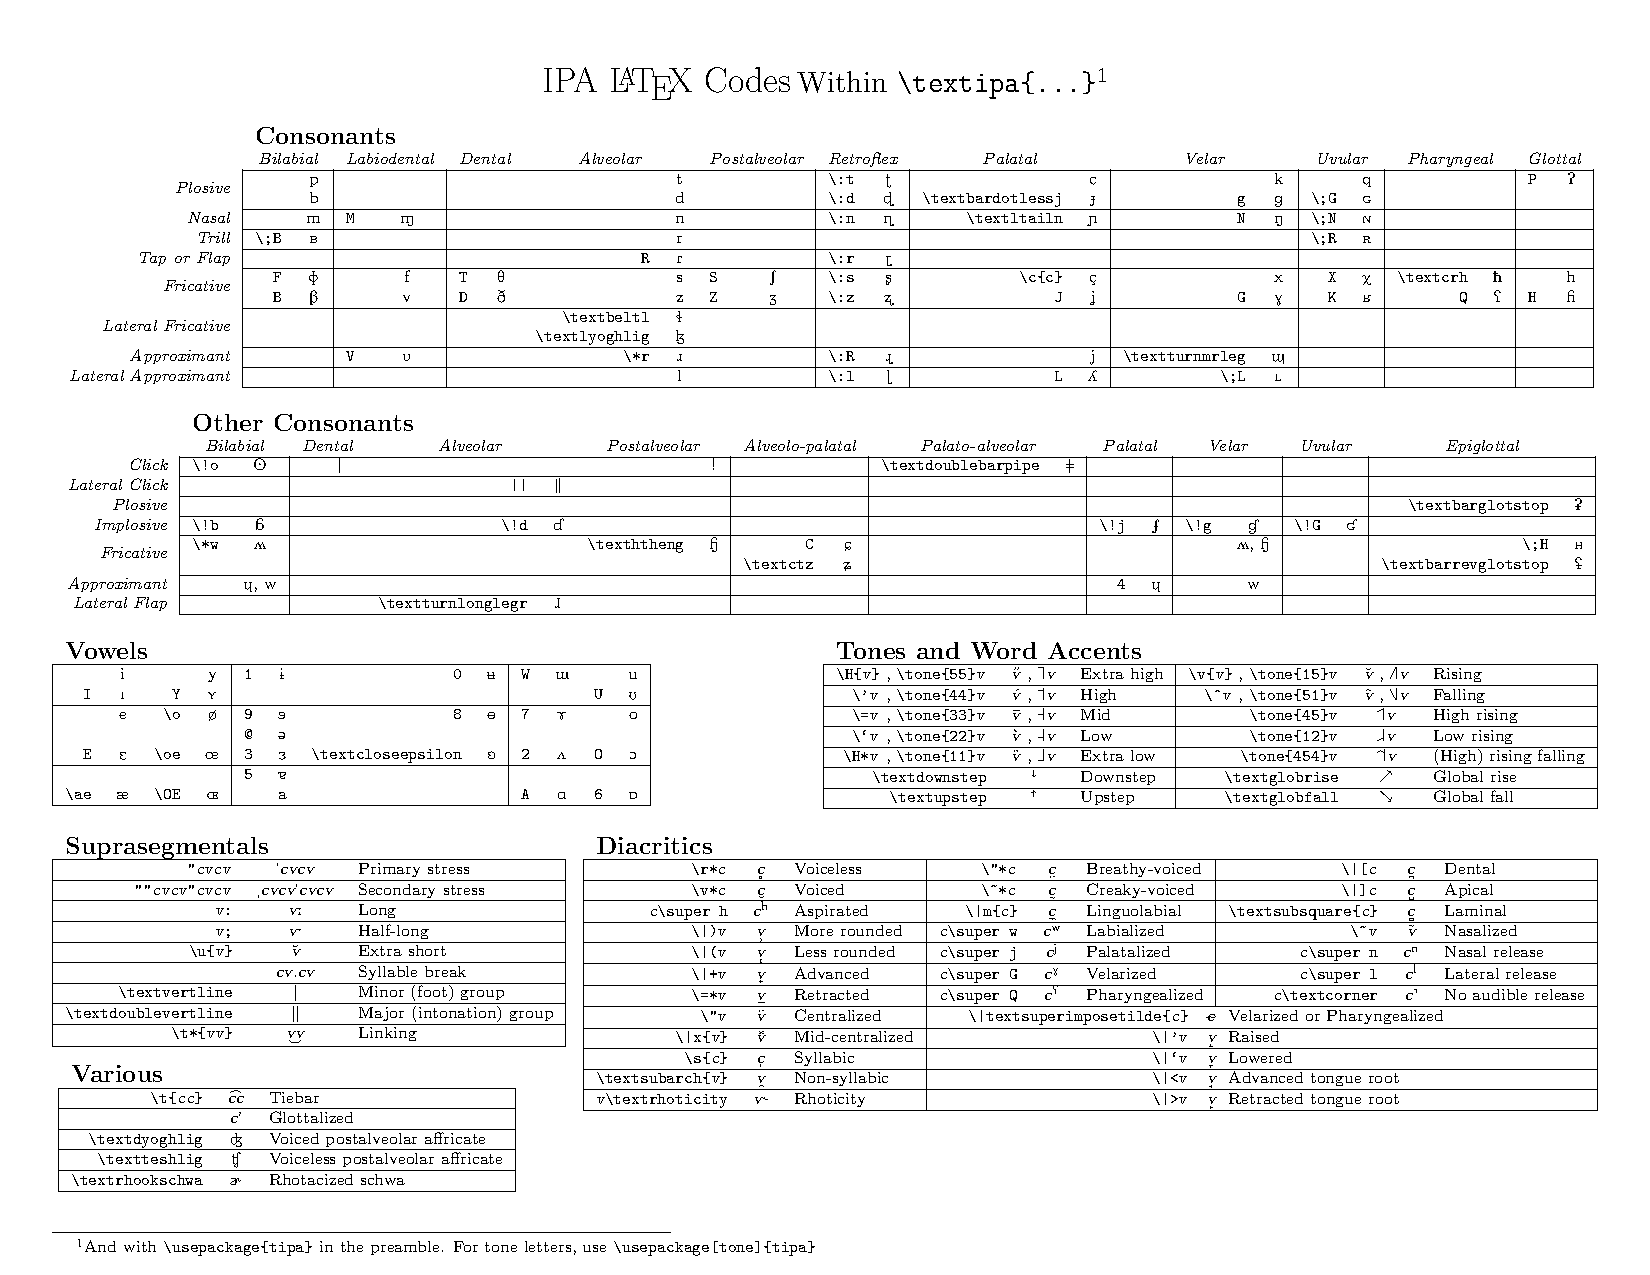
\includegraphics[width=\textwidth]
                     {figures/tipachart_mod.pdf}
  \caption{Tux.}
\end{figure}
\end{frame}



\begin{frame}[fragile]
\frametitle{Documento}
\framesubtitle{regras fonológicas}
  \scriptsize
  \begin{verbatim}
\usepackage{phonrule}
  
\phonb{\phonfeat{+stop \\ +consonant \\ +alveolar} }{[\textipa{R}]}
{\phonfeat{+vowel \\ +stressed} }{\phonfeat{+vowel \\ +stressed} }
  \end{verbatim}

  \begin{fmpage}{\textwidth}
\phonb{\phonfeat{+stop \\ +consonant \\ +alveolar} }{[\textipa{R}]}{\phonfeat{+vowel \\ +stressed} }{\phonfeat{+vowel \\ +stressed} }
  \end{fmpage}

\end{frame}


\begin{frame}[fragile]
\frametitle{Documento}
\framesubtitle{árvores sintáticas}
  \scriptsize
  \begin{columns}[c]
  \column{.5\textwidth}
  \begin{verbatim}
\begin{center}
\Tree [.S [.NP LaTeX ] [.VP [.V is ] 
  [.NP fun ] ] ]
\end{center}
  \end{verbatim}
  \column{.5\textwidth}
  \begin{fmpage}{\textwidth}
\begin{center}
\Tree [.S [.NP LaTeX ] [.VP [.V is ] [.NP fun ] ] ]
\end{center}
  \end{fmpage}
  \end{columns}
\end{frame}


\begin{frame}[fragile]
\frametitle{Documento}
\framesubtitle{Árvodre de dependência}
  \scriptsize
  \begin{verbatim}
   \usepackage{tikz-dependency}

    % In the document:
   \begin{dependency}[theme = simple]
   \begin{deptext}[column sep=1em]
      A \& hearing \& is \& scheduled \& on \& the \& issue \& today \& . \\
   \end{deptext}
   \deproot{3}{ROOT}
   \depedge{2}{1}{ATT}
   \depedge[edge start x offset=-6pt]{2}{5}{ATT}
   \depedge{3}{2}{SBJ}
   \depedge{3}{9}{PU}
   \depedge{3}{4}{VC}
   \depedge{4}{8}{TMP}
   \depedge{5}{7}{PC}
   \depedge[arc angle=50]{7}{6}{ATT}
   \end{dependency}
  \end{verbatim}
\end{frame}


\begin{frame}[fragile]
\frametitle{Documento}
\framesubtitle{Árvodre de dependência}
 
  \begin{fmpage}{\textwidth}
   \begin{dependency}[theme = simple]
   \begin{deptext}[column sep=1em]
      A \& hearing \& is \& scheduled \& on \& the \& issue \& today \& . \\
   \end{deptext}
   \deproot{3}{ROOT}
   \depedge{2}{1}{ATT}
   \depedge[edge start x offset=-6pt]{2}{5}{ATT}
   \depedge{3}{2}{SBJ}
   \depedge{3}{9}{PU}
   \depedge{3}{4}{VC}
   \depedge{4}{8}{TMP}
   \depedge{5}{7}{PC}
   \depedge[arc angle=50]{7}{6}{ATT}
   \end{dependency}
  \end{fmpage}

\end{frame}

\subsection{Notas e Citações}\label{sec:notascita}
\begin{frame}[fragile]
\frametitle{Notas de rodapé}
\framesubtitle{}
É fácil fazer uma nota de rodapé\footnote{Veja esta nota de rodapé.}.

\begin{verbatim}
É fácil fazer uma nota de 
rodapé\footnote{Veja esta nota de rodapé.}.
\end{verbatim}
\end{frame}

\begin{frame}[fragile]
\frametitle{Citações}
\framesubtitle{}
Citações pode ser feitas utilizardo o ambiente `quote'.
\begin{quote}
``Formatting is no substitute for writing''. (Leslie Lamport)
\end{quote}

\begin{scriptsize}
\begin{verbatim}
\begin{quote}
``Formatting is no substitute for writing''. (Leslie Lamport)
\end{quote}
\end{verbatim}
\end{scriptsize}
\end{frame}

\begin{frame}[fragile]
\frametitle{Citações}
\framesubtitle{outras formas de fazer citações}

Existem ainda vários pacotes para fazer citações, epígrafes, etc.
Veja alguns exemplos no \hrefcolor{https://www.overleaf.com/learn/latex/Typesetting_quotations}{Overleaf}.
\end{frame}


\subsection{Comandos}\label{sec:comandos}
\begin{frame}[fragile]
\frametitle{Comandos}
\framesubtitle{definindo novos comandos}

\begin{verbatim}
\newcommand{\R}{$\mathbb{R}$}
\end{verbatim}

Podemos definir novos comandos: \R.
É uma boa prática definí-los no preambulo do documento.

\end{frame}

\begin{frame}[fragile]
\frametitle{Comandos}
\framesubtitle{comandos com parâmetros}

\begin{verbatim}
\newcommand{\bb}[1]{$\mathbb{#1}$}

utilização:
\bb{C}, \bb{B}, \bb{D}
\end{verbatim}

Definimos acima um comando que possui um parâmetro.
Pode assim fácilmente gerar: \bb{C}, \bb{B}, \bb{D}.

\end{frame}



\subsection{Bibliografia}\label{sec:bibtex}
\begin{frame}[fragile]
\frametitle{Documento}
\framesubtitle{Bibliografia - como inserir uma obra e citá-la}
  \scriptsize
  \begin{columns}[c]
  \column{.5\textwidth}
  \begin{verbatim}
  @book{Knuth86,
  author    = {Donald E. Knuth},
  title     = {The TeXbook},
  publisher = {Addison-Wesley},
  year      = {1986},
  isbn      = {0-201-13447-0}
  }
  
  Citação no texto \cite{Knuth86}, \citep{Knuth86}.
  \end{verbatim} 
  \column{.5\textwidth}
  \begin{fmpage}{\textwidth}
  Citação no texto \cite{Knuth86}, \citep{Knuth86}.
  \end{fmpage}
  \end{columns}
\end{frame}


\begin{frame}[fragile]
\frametitle{Documento}
\framesubtitle{Atributos de um item de bibliografia}
  \scriptsize
  \begin{columns}[c]
  \column{.5\textwidth}
  \begin{verbatim}
@article{...,
    author  = "...",
    title   = "...",
    year    = "...",
    journal = "...",
    volume  = "...",
    number  = "...",
    pages   = "..."
}
  \end{verbatim} 
  \column{.5\textwidth}
\begin{verbatim}
@conference{...,
    author    = "...",
    title     = "...",
    booktitle = "...",
    %editor   = "...",
    %volume   = "...",
    %number   = "...",
    %series   = "...",
    %pages    = "...",
    %address  = "...",
    year      = "...",
    %month    = "...",
    %publisher= "...",
    %note     = "..."
}
\end{verbatim}
  \end{columns}
\end{frame}


\begin{frame}[fragile]
\frametitle{Documento}
\framesubtitle{Bibliografia - classes dos itens}
  \scriptsize
  \begin{columns}[c]
  \column{.5\textwidth}
  \begin{verbatim}
@inbook

@incollection

@inproceedings 

@mastersthesis
  \end{verbatim} 
  \column{.5\textwidth}
\begin{verbatim}
@misc 

@phdthesis 

@proceedings 

@techreport 

@unpublished 
\end{verbatim}
  \end{columns}
\end{frame}


\begin{frame}[fragile]
\frametitle{Documento}
\framesubtitle{Bibliografia - estilo}
  \scriptsize
  \begin{verbatim}
\bibliographystyle{apalike}
\bibliography{bibliografia}
  \end{verbatim}
  
  ver slide \pageref{bibliografia}.
\end{frame}






\begin{frame}[label={clsfile}]
\frametitle{Arquivo de classe de documento, arquivo de estilo e pacote}
\framesubtitle{.cls e .sty}
Veja o tutorial no  \hrefcolor{https://www.overleaf.com/learn/latex/Understanding_packages_and_class_files}{Overleaf}
\end{frame}
